\documentclass[aspectratio=169,11pt]{beamer}
% ==========================================================================
%  KSA lecture-slide theme  =  stock beamer "Boadilla"  +  KSA colour theme
%  brand colours sampled from the official KSA symbol mark:
%    Deep Prussian Blue  #2E3192   (지성 - intellect)
%    Golden Gray         #D6CBB1   (감성 - sensibility)
%  Engine: XeLaTeX.  Usage:
%    \documentclass[aspectratio=169,11pt]{beamer}
%    \input{../../theme/ksa-theme.tex}
%  Each deck lives in its own slides/kor/<deck>/ folder together with its
%  own images; ../../figs/ is kept only as a fallback for the shared cache.
% ==========================================================================

\usepackage{fontspec}
\usepackage{amsmath,amssymb}
\usepackage{graphicx}
\graphicspath{{figs/}{./}{../../../figs/}}
\usepackage{booktabs}
\usepackage{listings}
\usepackage{varwidth}

% ---- fonts (no ctex/xeCJK on this box -> fontspec drives CJK directly) -----
\defaultfontfeatures{Ligatures=TeX}
\setmainfont{Noto Sans CJK KR}
\setsansfont{Noto Sans CJK KR}
\setmonofont{Noto Sans Mono CJK KR}[Scale=0.92]

% ---- base theme: stock Boadilla ------------------------------------------
\usetheme{Boadilla}
\usefonttheme{professionalfonts}
\setbeamertemplate{navigation symbols}{}

% ---- KSA colour theme (recolour the stock theme) --------------------------
\definecolor{ksablue}{HTML}{2E3192}
\definecolor{ksabluedk}{HTML}{20226A}
\definecolor{ksagold}{HTML}{D6CBB1}
\definecolor{ksagolddk}{HTML}{A9976B}
\definecolor{ksared}{HTML}{C0392B}
\definecolor{ksagray}{HTML}{5B5B5B}

\setbeamercolor{structure}{fg=ksablue}
\setbeamercolor{alerted text}{fg=ksared}

\setbeamercolor{palette primary}{fg=white,           bg=ksablue}
\setbeamercolor{palette secondary}{fg=white,         bg=ksablue!85!black}
\setbeamercolor{palette tertiary}{fg=white,          bg=ksabluedk}
\setbeamercolor{titlelike}{fg=ksablue}
\setbeamercolor{frametitle}{fg=ksablue,bg=}
\setbeamercolor{title}{fg=ksablue}
\setbeamercolor{author}{fg=ksagray}
\setbeamercolor{institute}{fg=ksagray}
\setbeamercolor{block title}{fg=white,bg=ksablue}
\setbeamercolor{block body}{fg=black!85,bg=ksablue!6}
\setbeamercolor{item}{fg=ksablue}
\setbeamercolor{section in toc}{fg=black!85}

\setbeamerfont{frametitle}{series=\bfseries}
\setbeamerfont{title}{series=\bfseries}

% ---- footline:  KSA mark | "Made by ..." | n / N   (matches reference) ----
\newcommand{\ksacredit}{}
\setbeamertemplate{footline}{%
  \hbox{%
    \begin{beamercolorbox}[wd=.18\paperwidth,ht=2.6ex,dp=1.5ex,leftskip=1.1em]{}%
      \raisebox{-0.35ex}{\includegraphics[height=2.0ex]{ksa-logo.png}}%
    \end{beamercolorbox}%
    \begin{beamercolorbox}[wd=.64\paperwidth,ht=2.6ex,dp=1.5ex,center]{}%
      {\scriptsize\color{ksagray}\ksacredit}%
    \end{beamercolorbox}%
    \begin{beamercolorbox}[wd=.18\paperwidth,ht=2.6ex,dp=1.5ex,rightskip=1.1em]{}%
      \hfill{\scriptsize\color{ksablue}\insertframenumber\,/\,\inserttotalframenumber}%
    \end{beamercolorbox}%
  }%
  \vskip2pt
}

% ---- section divider: stock \sectionpage, KSA-coloured -------------------
\setbeamertemplate{section page}{%
  \begingroup\centering
    {\color{ksagolddk}\rule{0.16\paperwidth}{1pt}}\par\vskip1.0em
    {\usebeamerfont{title}\color{ksablue}\insertsectionhead\par}\vskip1.0em
    {\color{ksagolddk}\rule{0.16\paperwidth}{1pt}}\par
  \endgroup
}
\AtBeginSection[]{\begin{frame}[plain,noframenumbering]\vfill\sectionpage\vfill\end{frame}}

% ---- code listings ------------------------------------------------------------
\lstdefinestyle{ksa}{%
  basicstyle=\ttfamily\scriptsize,
  keywordstyle=\color{ksablue}\bfseries,
  commentstyle=\color{ksagray}\itshape,
  stringstyle=\color{ksagolddk},
  numberstyle=\tiny\color{ksagray},
  backgroundcolor=\color{ksablue!6},
  frame=leftline, framerule=1.4pt, rulecolor=\color{ksablue},
  xleftmargin=1em, aboveskip=0.8em, belowskip=0.4em,
  showstringspaces=false, breaklines=true, language=Python,
}
\lstset{style=ksa}

% ---- handy macros -----------------------------------------------------------
\newcommand{\kb}[1]{\textbf{\color{ksablue}#1}}   % blue keyword
\newcommand{\kq}[1]{\textbf{\color{ksared}#1}}    % red key-question

\setbeamerfont{title}{series=\bfseries,size=\fontsize{24}{30}\selectfont}
\setbeamerfont{subtitle}{series=\bfseries,size=\fontsize{14}{18}\selectfont}
\setbeamerfont{author}{size=\normalsize}
\setbeamerfont{institute}{size=\small}
\graphicspath{{figs/}{../../../../assets/}}
\makeatletter
\newcommand{\markpage}[1]{\protected@write\@auxout{}{\string\newlabel{#1}{{\the\c@framenumber}{}}}\hypertarget{#1}{}}
\newcommand{\pref}[1]{\hyperlink{#1}{\textcolor{ksagolddk}{(p.\ref{#1})}}}
\makeatother

\renewcommand{\ksacredit}{Machine Learning 1 \,\textperiodcentered\, 결정 트리}
\title{결정 트리 (Decision Tree)}
\subtitle{스무고개처럼 질문으로 나누기, 좋은 질문 고르기}
\author{Machine Learning 1}
\institute{한국과학영재학교 (KSA)}
\date{}
\begin{document}
\begin{frame}[plain,noframenumbering]\titlepage\end{frame}

% --- 오늘의 질문
\begin{frame}{오늘의 질문}
\vfill
\centering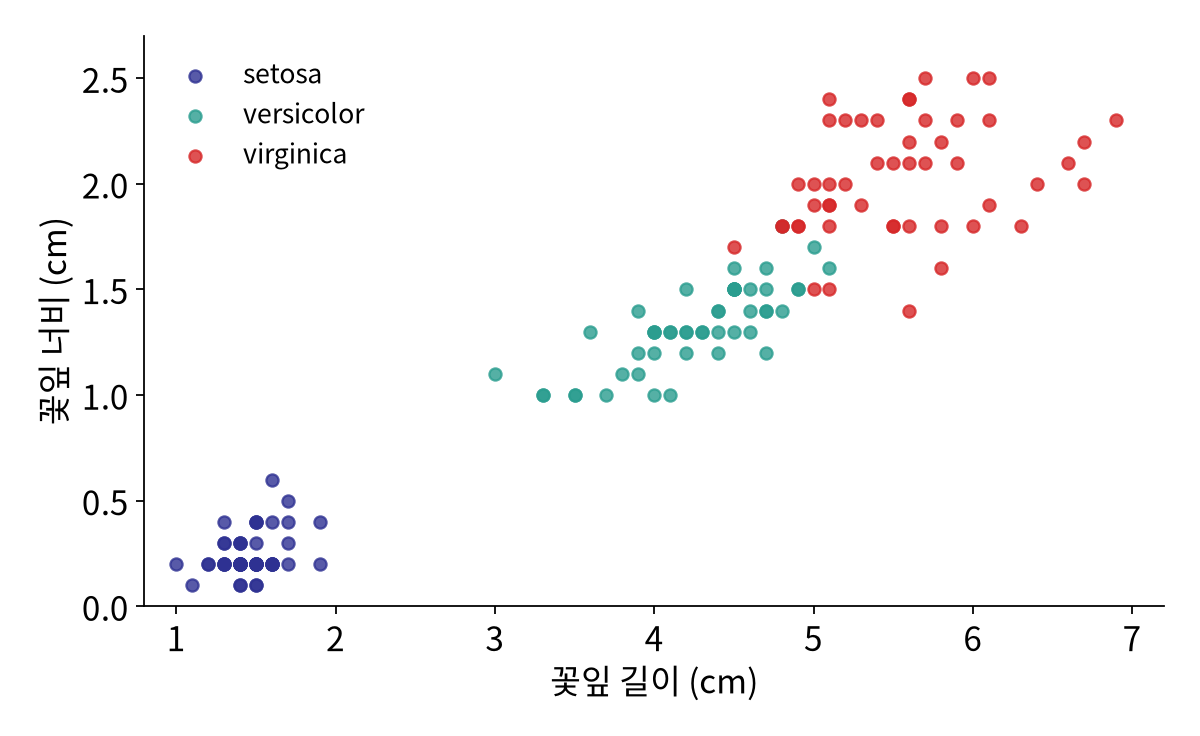
\includegraphics[width=0.56\linewidth]{dt_hook.png}\par\vskip0.2em
{\large 붓꽃 150송이, 3종. 꽃잎 길이와 너비만 보고 \kq{예 · 아니오 질문 몇 개로 가를 수 있을까?}}
\vfill
\note{붓꽃 150송이입니다. setosa, versicolor, virginica 세 종이 50송이씩 있고, 꽃잎의 길이와 너비를 쟀습니다. 이 두 숫자만 보고 종을 맞히고 싶습니다. 오늘은 스무고개처럼 예, 아니오로 답할 질문을 몇 개 이어 가며 데이터를 나누는 방법, 결정 트리를 배웁니다. 선형회귀나 SVM처럼 식을 세우지 않고, 사람이 읽을 수 있는 규칙을 만든다는 점이 특징입니다.}
\end{frame}

% --- 좋은 질문
\begin{frame}{질문마다 나뉘는 정도가 다르다}
\vfill
\centering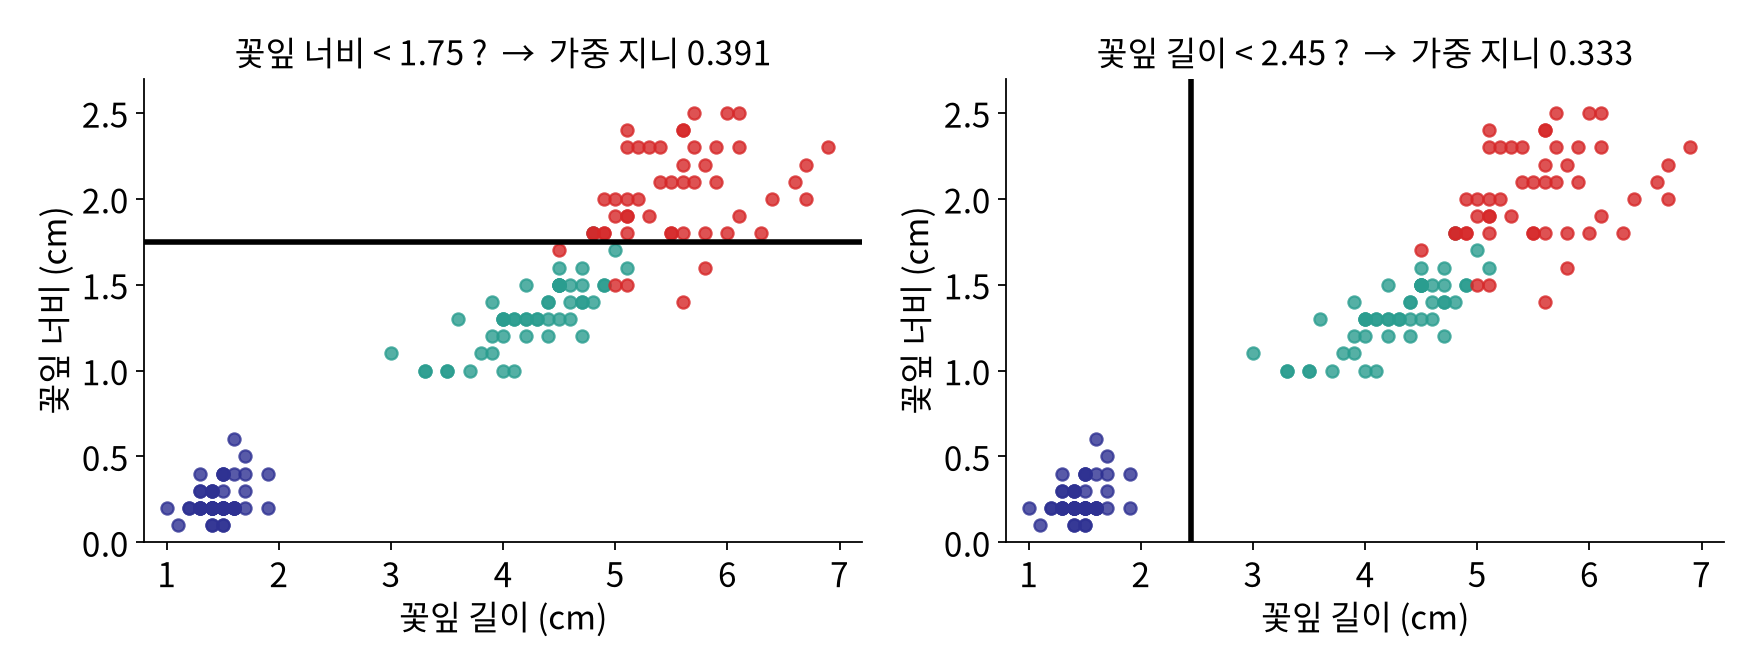
\includegraphics[width=0.86\linewidth]{dt_candidates.png}\par\vskip0.2em
{\large 왼쪽: 양쪽 다 여전히 섞여 있다 \qquad 오른쪽: 한쪽이 \kb{setosa 만 50송이}}\\[0.2em]
{\large 좋은 질문 = 나눈 뒤 \textbf{덜 섞이게} 만드는 질문}
\vfill
\note{첫 질문을 어떻게 고를까요? 두 후보를 봅니다. 왼쪽은 꽃잎 너비가 1.75보다 작으냐는 질문인데, 아래쪽에 setosa와 versicolor, 그리고 virginica 몇 송이가 섞여 있습니다. 오른쪽은 꽃잎 길이가 2.45보다 짧으냐는 질문인데, 왼쪽에는 setosa 50송이만 깨끗하게 남습니다. 오른쪽이 더 좋은 질문입니다. 나눈 뒤 덜 섞이게 만드니까요. 이 섞인 정도를 숫자로 재는 방법이 필요합니다.}
\end{frame}

% --- 지니
\begin{frame}{섞인 정도를 숫자로: 지니 불순도}
\markpage{gini}
\vfill
\centering
{\LARGE\[ \text{Gini} = 1 - \sum_{k} p_k^2 \]}\vskip0.2em
{\small $p_k$: 그 칸에서 종 $k$ 의 비율}\vskip0.6em
\renewcommand{\arraystretch}{1.3}
{\large\begin{tabular}{lll}
한 종만 & $1 - 1^2$ & \kb{0} \quad (깨끗하다)\\
두 종 반반 & $1 - 0.5^2 - 0.5^2$ & 0.5\\
세 종 $\frac13$ 씩 & $1 - 3 \times \left(\frac13\right)^2$ & \kq{0.667} \quad (붓꽃 150송이 전체)
\end{tabular}}\vskip0.4em
{\small 뜻: 칸에서 아무 꽃이나 하나 골라, 비율대로 아무렇게나 이름을 붙이면 틀릴 확률}
\vfill
\note{섞인 정도를 재는 가장 흔한 방법이 지니 불순도입니다. 1에서 각 종의 비율의 제곱을 빼면 됩니다. 한 종만 있으면 1 빼기 1, 0입니다. 깨끗합니다. 두 종이 반반이면 1 빼기 0.25 빼기 0.25, 0.5입니다. 세 종이 3분의 1씩이면 0.667, 붓꽃 150송이 전체가 이 상태입니다. 뜻을 붙이면, 칸에서 꽃 하나를 고르고 칸의 비율대로 아무렇게나 이름을 붙였을 때 틀릴 확률입니다. 다음 시간에는 지니 대신 엔트로피로 재는 방법을 봅니다.}
\end{frame}

% --- 손으로
\begin{frame}{손으로 한 번: 어느 질문이 더 좋은가}
\vfill
\centering
{\large 나눈 뒤의 불순도 = 양쪽 지니를 \textbf{꽃 수로 가중 평균}}\vskip0.5em
{\Large\[ \text{꽃잎 길이} < 2.45: \quad \frac{50}{150}\cdot 0 + \frac{100}{150}\cdot 0.5 = \kb{0.333} \]}
{\Large\[ \text{꽃잎 너비} < 1.75: \quad \frac{104}{150}\cdot 0.545 + \frac{46}{150}\cdot 0.043 = 0.391 \]}\vskip0.3em
{\large 0.667 에서 \kb{0.333} 만큼 줄인 꽃잎 길이 질문을 고른다 \quad (줄어든 양 = 정보 이득)}
\vfill
\note{두 질문을 숫자로 비교해 봅니다. 나눈 뒤의 불순도는 양쪽의 지니를 꽃 수로 가중 평균한 값입니다. 꽃잎 길이 2.45로 나누면 왼쪽 50송이는 setosa뿐이라 지니 0, 오른쪽 100송이는 versicolor와 virginica 반반이라 0.5입니다. 가중 평균은 3분의 2 곱하기 0.5, 0.333입니다. 꽃잎 너비 1.75로 나누면 왼쪽 104송이는 세 종이 섞여 지니 0.545, 오른쪽 46송이는 0.043, 가중 평균 0.391입니다. 원래 0.667에서 더 많이 줄인 꽃잎 길이 질문을 고릅니다. 이렇게 줄어든 양을 정보 이득이라고 부릅니다.}
\end{frame}

% --- 모든 기준값
\begin{frame}{후보를 전부 재 본다}
\vfill
\centering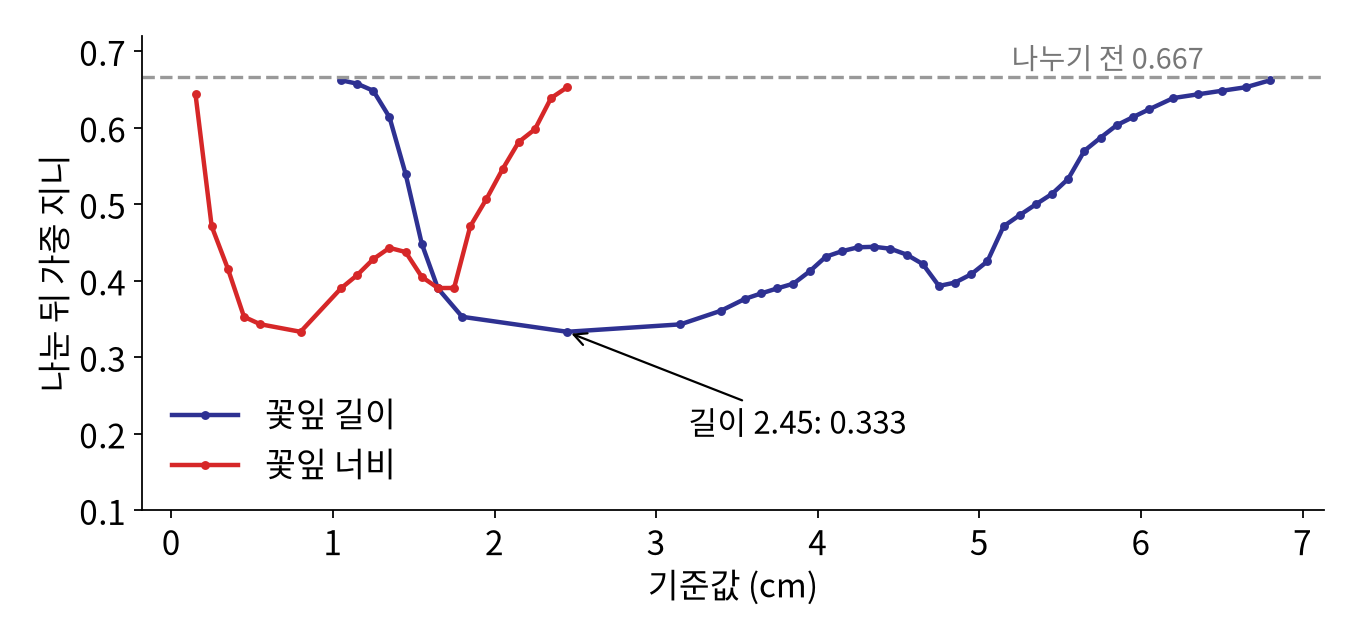
\includegraphics[width=0.6\linewidth]{dt_sweep.png}\par\vskip0.2em
{\large 특징마다 정렬한 값들의 \textbf{중간점}이 모두 후보 \quad $\to$ 가장 낮은 곳을 고른다}\\[0.2em]
{\small 꽃잎 길이 2.45 와 꽃잎 너비 0.8 이 똑같이 0.333 (둘 다 setosa 만 깔끔히 떼어 낸다)}
\vfill
\note{실제로는 후보를 전부 재 봅니다. 특징마다 값을 정렬하고, 이웃한 두 값의 중간점을 모두 기준값 후보로 삼아 가중 지니를 계산합니다. 파란 선이 꽃잎 길이, 빨간 선이 꽃잎 너비입니다. 가장 낮은 곳은 0.333이고, 꽃잎 길이 2.45와 꽃잎 너비 0.8이 똑같이 이 값을 냅니다. 둘 다 setosa만 깔끔하게 떼어 내니까요. 동점이면 어느 쪽이든 괜찮습니다. 특징 수 곱하기 데이터 수만큼만 재면 되니 컴퓨터에게는 쉬운 일입니다.}
\end{frame}

% --- 두 번째 질문
\begin{frame}{남은 칸에서 같은 일을 반복한다}
\markpage{tree}
\vfill
\centering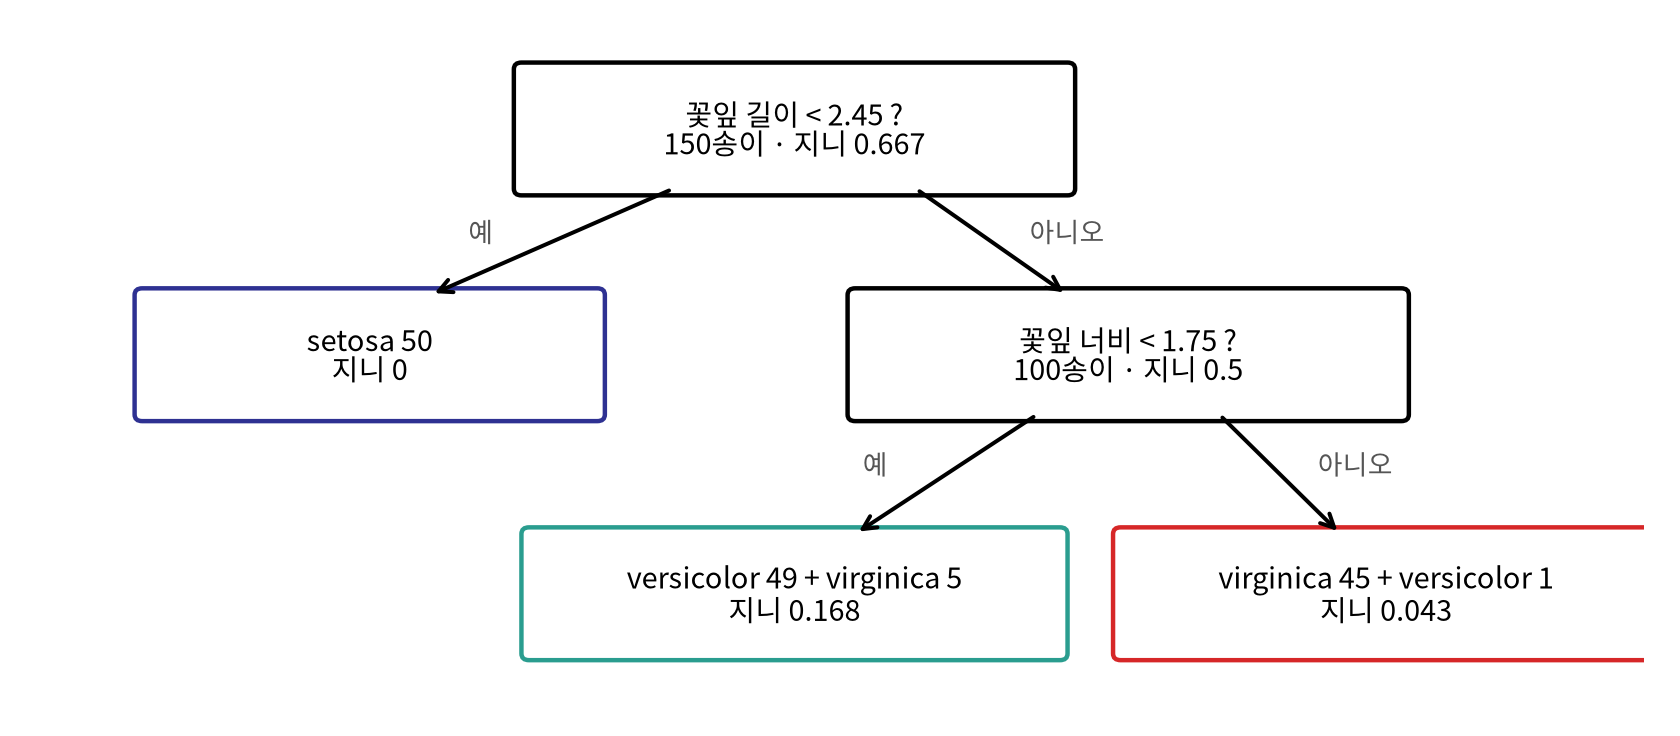
\includegraphics[width=0.74\linewidth]{dt_tree.png}\par\vskip0.1em
{\large 남은 100송이를 꽃잎 너비 1.75 로 \quad 가중 지니 0.5 $\to$ \kb{0.11} \quad 질문의 끝 = \textbf{잎 (leaf)}}
\vfill
\note{setosa가 떨어져 나간 뒤, 남은 100송이에서 같은 일을 반복합니다. 이번에는 꽃잎 너비 1.75가 가장 좋은 질문입니다. 왼쪽에는 versicolor 49송이와 virginica 5송이, 오른쪽에는 virginica 45송이와 versicolor 1송이가 남습니다. 지니가 0.5에서 0.11로 줄었습니다. 한 종이 대부분을 차지하면 여기서 멈춥니다. 더 이상 질문하지 않는 끝을 잎이라고 부르고, 잎에서는 가장 많은 종으로 답합니다. 이렇게 나뭇가지처럼 갈라지는 모양이라 결정 트리라고 부릅니다.}
\end{frame}

% --- 예측
\begin{frame}{새 꽃은 질문을 따라 내려간다}
\vfill
\centering
{\Large 꽃잎 길이 5.1 cm, 너비 1.8 cm 인 새 꽃}\\[1.0em]
{\Large 길이 $< 2.45$? \textbf{아니오} \quad $\to$ \quad 너비 $< 1.75$? \textbf{아니오} \quad $\to$ \quad \kq{virginica}}\\[1.0em]
{\large 질문 2번이면 답이 나온다 \quad 그리고 \textbf{왜} 그렇게 답했는지 사람이 읽을 수 있다}\\[0.4em]
{\small 거리를 재지 않으니 단위가 달라도 상관없다 (표준화가 필요 없다)}
\vfill
\note{새 꽃이 오면 질문을 따라 내려가기만 하면 됩니다. 꽃잎 길이 5.1, 너비 1.8인 꽃은 첫 질문에 아니오, 두 번째 질문에 아니오라서 virginica입니다. 질문 두 번이면 답이 나오고, 왜 그렇게 답했는지 사람이 그대로 읽을 수 있습니다. 꽃잎이 길고 넓어서 virginica라고요. 의사나 은행처럼 판단 이유를 설명해야 하는 곳에서 결정 트리를 좋아하는 이유입니다. 또 거리를 재지 않고 한 특징씩 크기만 비교하니, kNN과 달리 단위가 달라도 표준화가 필요 없습니다.}
\end{frame}

% --- 깊게 키우면
\begin{frame}{끝까지 키우면}
\vfill
\centering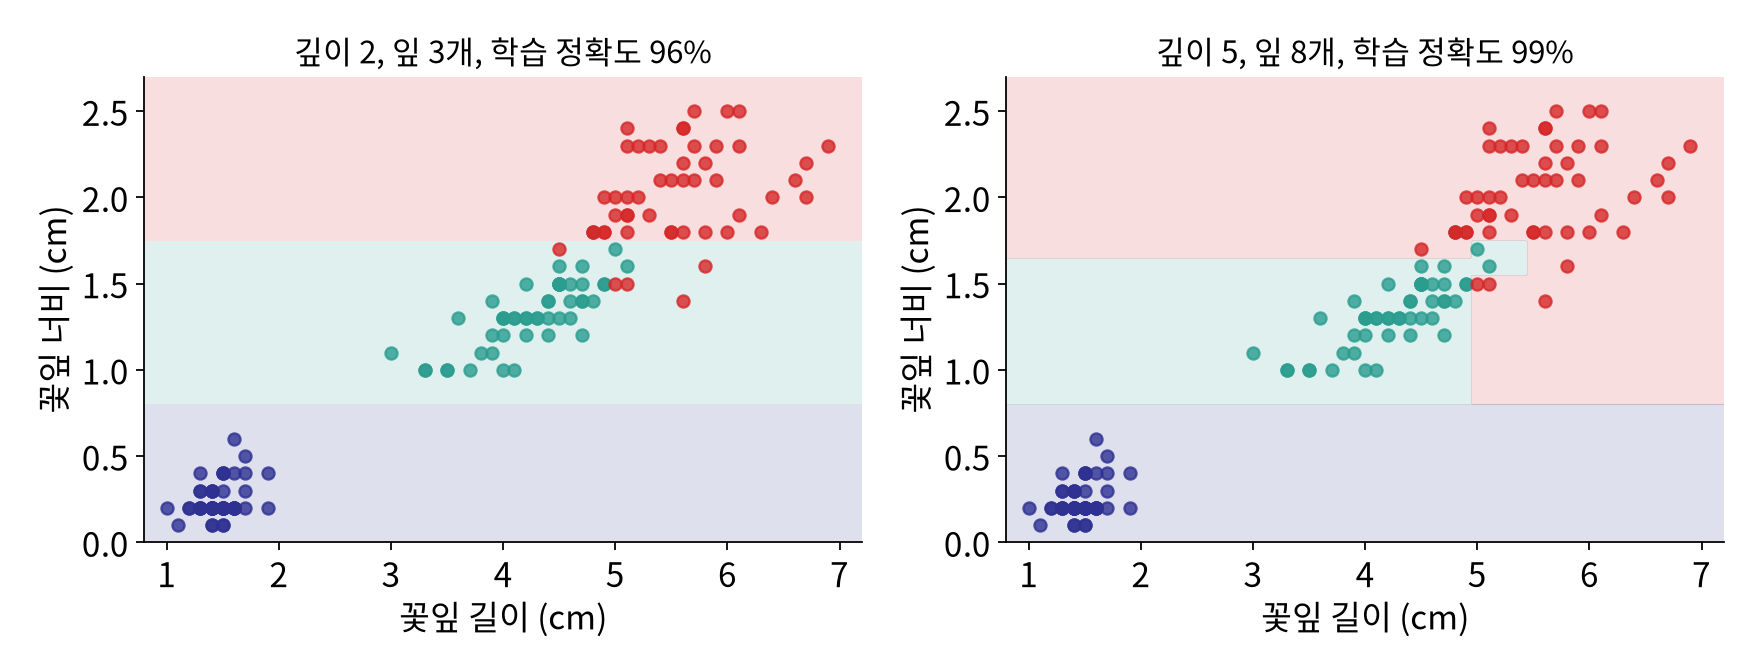
\includegraphics[width=0.86\linewidth]{dt_boundary.png}\par\vskip0.2em
{\large 깊이 2: 잎 3개, 학습 96\% \quad 끝까지: 잎 8개, 학습 \kq{99\%} (경계의 몇 송이를 외운다)}
\vfill
\note{질문을 멈추지 않고 끝까지 키우면 어떻게 될까요? 왼쪽은 깊이 2, 잎 3개로 학습 정확도 96퍼센트입니다. 오른쪽은 끝까지 키운 트리로 깊이 5, 잎 8개, 학습 정확도 99퍼센트입니다. 그런데 늘어난 잎들은 versicolor와 virginica 경계에 걸친 몇 송이를 맞히려고 작은 칸을 따로 만든 겁니다. 측정 오차일 수도 있는 몇 송이를 외운 셈입니다. 붓꽃은 깨끗한 데이터라 피해가 작지만, 섞인 데이터에서는 문제가 커집니다.}
\end{frame}

% --- Pima
\begin{frame}{섞인 데이터에서는: 깊을수록 시험에서 나빠진다}
\markpage{depth}
\vfill
\centering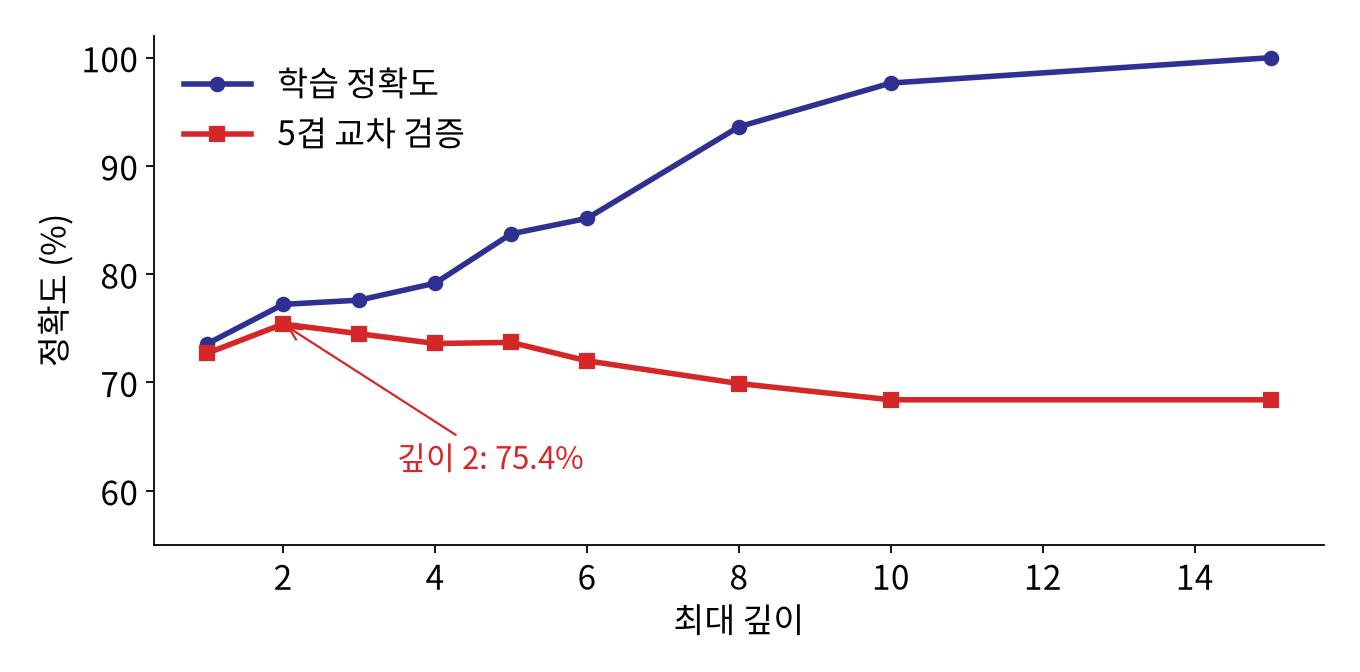
\includegraphics[width=0.6\linewidth]{dt_depth.png}\par\vskip0.2em
{\large 당뇨병 768명 (검사값 8개): 끝까지 키우면 학습 \kq{100\%} (잎 130개), 교차 검증 \kq{68.6\%}}\\[0.2em]
{\large 깊이 2: 학습 77\%, 교차 검증 \kb{75.4\%} \quad $\to$ \textbf{최대 깊이}도 교차 검증으로 고른다}
\vfill
\note{섞인 데이터의 예로 당뇨병 환자 768명을 봅니다. 혈당, BMI, 나이 같은 검사값 8개로 당뇨병을 맞힙니다. 트리를 끝까지 키우면 잎이 130개가 되고 학습 정확도는 100퍼센트입니다. 모든 환자를 외웠습니다. 그런데 5겹 교차 검증 정확도는 68.6퍼센트로 떨어집니다. 깊이를 2로 제한하면 학습 정확도는 77퍼센트지만 교차 검증은 75.4퍼센트로 가장 높습니다. 트리의 최대 깊이도 지금까지 본 손잡이처럼 교차 검증으로 고릅니다. 잎 하나에 최소 몇 개가 있어야 하는지를 정하는 min_samples_leaf도 같은 역할을 합니다.}
\end{frame}

% --- 장단점
\begin{frame}{결정 트리의 장점과 약점}
\vfill
\centering
\renewcommand{\arraystretch}{1.5}
{\large\begin{tabular}{ll}
\kb{장점} & 사람이 읽을 수 있는 규칙 \quad 표준화 불필요 \quad 숫자 · 범주 특징 섞어 써도 된다\\
\kq{약점} & 깊으면 과대적합 \quad 데이터가 조금만 바뀌어도 트리 모양이 크게 바뀐다\\
 & 경계가 축에 평행한 계단 모양뿐
\end{tabular}}\vskip1.0em
{\large 약점을 메우는 방법: 트리를 \textbf{많이} 만들어 투표한다 $\to$ 랜덤 포레스트, GBDT}
\vfill
\note{정리해 보면, 결정 트리는 사람이 읽을 수 있는 규칙을 만들고, 표준화가 필요 없고, 숫자와 범주 특징을 섞어 써도 됩니다. 약점도 분명합니다. 깊으면 쉽게 과대적합되고, 데이터가 조금만 바뀌어도 첫 질문이 달라지면서 트리 모양이 크게 바뀝니다. 불안정하다는 뜻입니다. 그리고 한 번에 한 특징만 보니 경계가 축에 평행한 계단 모양뿐입니다. 이 약점을 메우는 방법이 트리를 많이 만들어 투표하는 것이고, 이번 주 뒤에 랜덤 포레스트와 GBDT로 이어집니다.}
\end{frame}

% --- 문제풀이
\begin{frame}{문제풀이}
\vfill
\begin{enumerate}
\item 한 칸에 사과 6, 귤 2 가 있다. 지니 불순도는?\vskip0.8em
\item 사과 4 · 귤 4 인 칸을 질문 A 는 (사과 4 · 귤 1) / (귤 3) 으로, 질문 B 는 (사과 2 · 귤 2) / (사과 2 · 귤 2) 로 나눈다. 각각의 가중 지니는? 어느 질문을 고르나?\vskip0.8em
\item 학습 정확도 100\%, 교차 검증 정확도 65\% 인 결정 트리. 무엇을 바꿔 보겠나?
\end{enumerate}
\vfill
\note{1번 답. 비율이 0.75와 0.25라서 1 빼기 0.5625 빼기 0.0625, 0.375입니다. 2번 답. 질문 A의 왼쪽은 비율 0.8과 0.2로 지니 0.32, 오른쪽은 귤만 있어 0, 가중 평균은 8분의 5 곱하기 0.32로 0.2입니다. 질문 B는 양쪽 다 반반이라 0.5 그대로입니다. 전혀 줄지 않았습니다. A를 고릅니다. 3번 답. 과대적합이니 최대 깊이를 줄이거나 min_samples_leaf를 키우고, 교차 검증으로 값을 고릅니다.}
\end{frame}

% --- 실습
\begin{frame}{실습}
\vfill
\centering\begin{tabular}{rl}
\large 1 & 지니 불순도와 가장 좋은 질문 찾기 직접 구현 $\to$ 붓꽃 0.333, 0.11 재현\\[0.5em]
\large 2 & scikit-learn 트리를 그려 보고, 새 꽃 판정 경로 따라가기\\[0.5em]
\large 3 & 실제 데이터: 타이타닉 891명 생존 예측, 최대 깊이를 교차 검증으로
\end{tabular}\vskip1em
Iris (Fisher, 1936) · Titanic (Kaggle / seaborn-data) \\[0.4em]\href{https://colab.research.google.com/github/SuminHan/book-ml/blob/main/slides/v2/ml1/week07/decision_tree/lab/decision_tree.ipynb}{\textcolor{ksagolddk}{▶ Colab에서 실습 노트북 열기}}
\vfill
\note{실습은 세 부분입니다. 첫째, 지니 불순도와 가장 좋은 질문을 찾는 함수를 직접 구현해서 붓꽃의 0.333과 0.11을 재현합니다. 둘째, scikit-learn으로 만든 트리를 그림으로 그려 보고, 새 꽃이 어느 길로 내려가는지 따라갑니다. 셋째, 타이타닉 승객 891명의 생존 여부를 결정 트리로 예측하고, 최대 깊이를 교차 검증으로 고른 뒤 어떤 질문이 먼저 나오는지 읽어 봅니다.}
\end{frame}

% --- 정리
\begin{frame}{정리}
\vfill
\centering\large\begin{tabular}{l}
\textbf{결정 트리} \quad 예 · 아니오 질문으로 칸을 나누고, 잎에서 다수결\\[0.5em]
좋은 질문 = 가중 \kb{지니 불순도} ($1 - \sum p_k^2$) 를 가장 많이 줄이는 질문\\[0.5em]
후보를 전부 재고 고른 뒤, 남은 칸에서 반복\\[0.5em]
깊으면 과대적합 $\to$ \textbf{최대 깊이}를 교차 검증으로 \quad 불안정 $\to$ 숲으로
\end{tabular}
\vfill
\note{정리합니다. 결정 트리는 예, 아니오 질문으로 칸을 나누고 잎에서 다수결로 답합니다. 좋은 질문은 나눈 뒤의 가중 지니 불순도를 가장 많이 줄이는 질문이고, 특징과 기준값 후보를 전부 재서 고른 뒤 남은 칸에서 반복합니다. 깊이 키울수록 과대적합되니 최대 깊이를 교차 검증으로 고르고, 데이터에 따라 모양이 잘 바뀌는 불안정함은 트리를 여러 개 모은 숲으로 해결합니다. 다음 시간에는 지니 대신 쓰는 또 다른 섞임 측정, 섀넌 엔트로피를 배웁니다.}
\end{frame}
\end{document}
